\chapter {Analysis and Design}
The file format is divided into the two autonomous parts DATA and METADATA, which relate to each other, but could be read or written separately. The both parts are stored in one \gls{hdf5} container.

The data part stores all recorded binary data and the basic information about measuring for correct representation of measured data (Sampling interval, resolution and resolution unit). This section includes data from the eeg \ref{eeg}, vhdr \ref{vhdr} and vmrk \ref{vmrk} files. The file structure is defined by the NIX file model - (Figure~\ref{NIX_scheme}). I also use the same terminology and the file structure. However our model - EEGBase model was simplified for our needs. More specific description follows in Section~\ref{section_data}.

Java was selected as a programming language for program developing, because there is already parser of Brain Vision formats developed and also the EEGBase portal is written in Java. There is effort to include the export program into the EEGBase portal for easy export.



\section{Current Formats Comparison}
The comparison of the selected file formats is in Table~\ref{format_comparsion1}. Formats in the comparison were selected, because they use \gls{hdf5} and their model is open. The close models could be limited by licenses and their modifications could be limited.
The valuated criteria are: 
\begin{itemize}
\item \textbf{Proprietary} - the format is open source / closed
\item \textbf{Data terminology} - terminology for data (and necessary metadata) is defined
\item \textbf{Data ontology} - ontology for data is defined
\item \textbf{Metadata terminology} - terminology for metadata is defined
\item \textbf{Metadata ontology} - terminology for metadata is defined
\item \textbf{Portability} - the format has an \gls{api} for different languages, platforms
\item \textbf{Java API} - the format has Java \gls{api} (my program is in Java)
\item \textbf{Extensibility of model} - the data and metadata models are extensible
\item \textbf{Documentation of format} - the file format documentation and its availability
\end{itemize}
I evaluated formats with three grades compared to our needs. One is best, minus one is worst. The evaluation is subjective even though I tried to be as objective as possible.

\begin{table}[h]
	\caption{The current formats comparison.} 
	\scalebox{0.95}{
	\tabcolsep=0.13cm
	\begin{tabular}{| p{2,7cm} |c|c|c|c|c|c|c|}
		\hline \textbf{Format} &	\textbf{Ovation} 	& \textbf{EDF+} & \textbf{NeXus} & \textbf{NEO} & \textbf{neuroHDF} & \textbf{NIX} & \textbf{epHDF} \\ 
		\hline
		\hline Proprietary  	& -1 	& 1	 	& 1 & 1 & 1 & 1 & 1 \\ 
		\hline Data 
		
		terminology 		& 1 	& 1 	& 0  & 1 & 0 & 1 & 1  \\ 
		\hline Data 
		
		ontology 			& 1 	& 1 	& 0  & 1 & 1 & 1 & 1  \\ 
		\hline Metadata 
		
		terminology 		& 1 	& 1 	& -1  & 0 & -1 & 1 & 1  \\ 
		\hline Metadata 
		
		ontology 			& 1 	& 1 	& -1  & 0 & -1 & 1 & 1  \\ 						
		\hline Portability  & 0 	& 1 	& 1 & 1& 1 & 0 & -1  \\ 
		\hline Java API  	& -1 	& 1 	& 1 & -1  & -1 & -1 & -1\\ 
		\hline Extensibility & 0 	& -1 	& -1  & 0 & 0 & 1 & 1 \\ 
		\hline Documentation & 1 	& 1 	& 1  & 1 & 0 & 1 & 0 \\ 
		\hline 
		
	\end{tabular}  
}
\label{format_comparsion1}	
\end{table}

NIX and epHDF look like the best models. Both these models are supported by \gls{incf}.The NIX project offers only C++ \gls{api} and epHDF is only a standard for file format. Because my effort was integrate program for exporting measured data into the EEGBase portal \cite{eegportal}, which is in Java, I choose Java as the programming language for my program. The HDF Group provides Java \gls{api} for read and write \gls{hdf} files so I was able to create my own program that writes data in the \gls{hdf5} container. Because the NIX model is better commented and provides \gls{api}, I choose NIX as a initial solution for EEGBase format.

\section{Data Model}
\label{section_data}
The data model is based on the NIX data model (Figure~\ref{NIX_scheme} and Section~\ref{nixsection}). The NIX model is able to save data from any electrophysiology experiment. But for \gls{eeg} experiments the NIX model is too general. So I used only necessary parts of the model and other sections were omitted. The omitted parts are in the NIX model optional, so my format is compatible with the NIX definition. My data model is described in Figure~\ref{format_scheme}. The data model uses the NIX scheme of Block, DataArray, MultiTag, DataTag and SimpleTag. The Block is used to divide measuring, DataArray stores raw data of signals and stimuli and MultiTag stores stimuli information and DataTag contains \gls{eeg} channel information. DataArrays are divided for better distribution in my model to SIGNAL and MARKER parts. Also, the names of DataArrays correspond to names of channels. These adjustments allow better human readability and do not influence information or the model compatibility.

\begin{figure}
	\begin{center}
		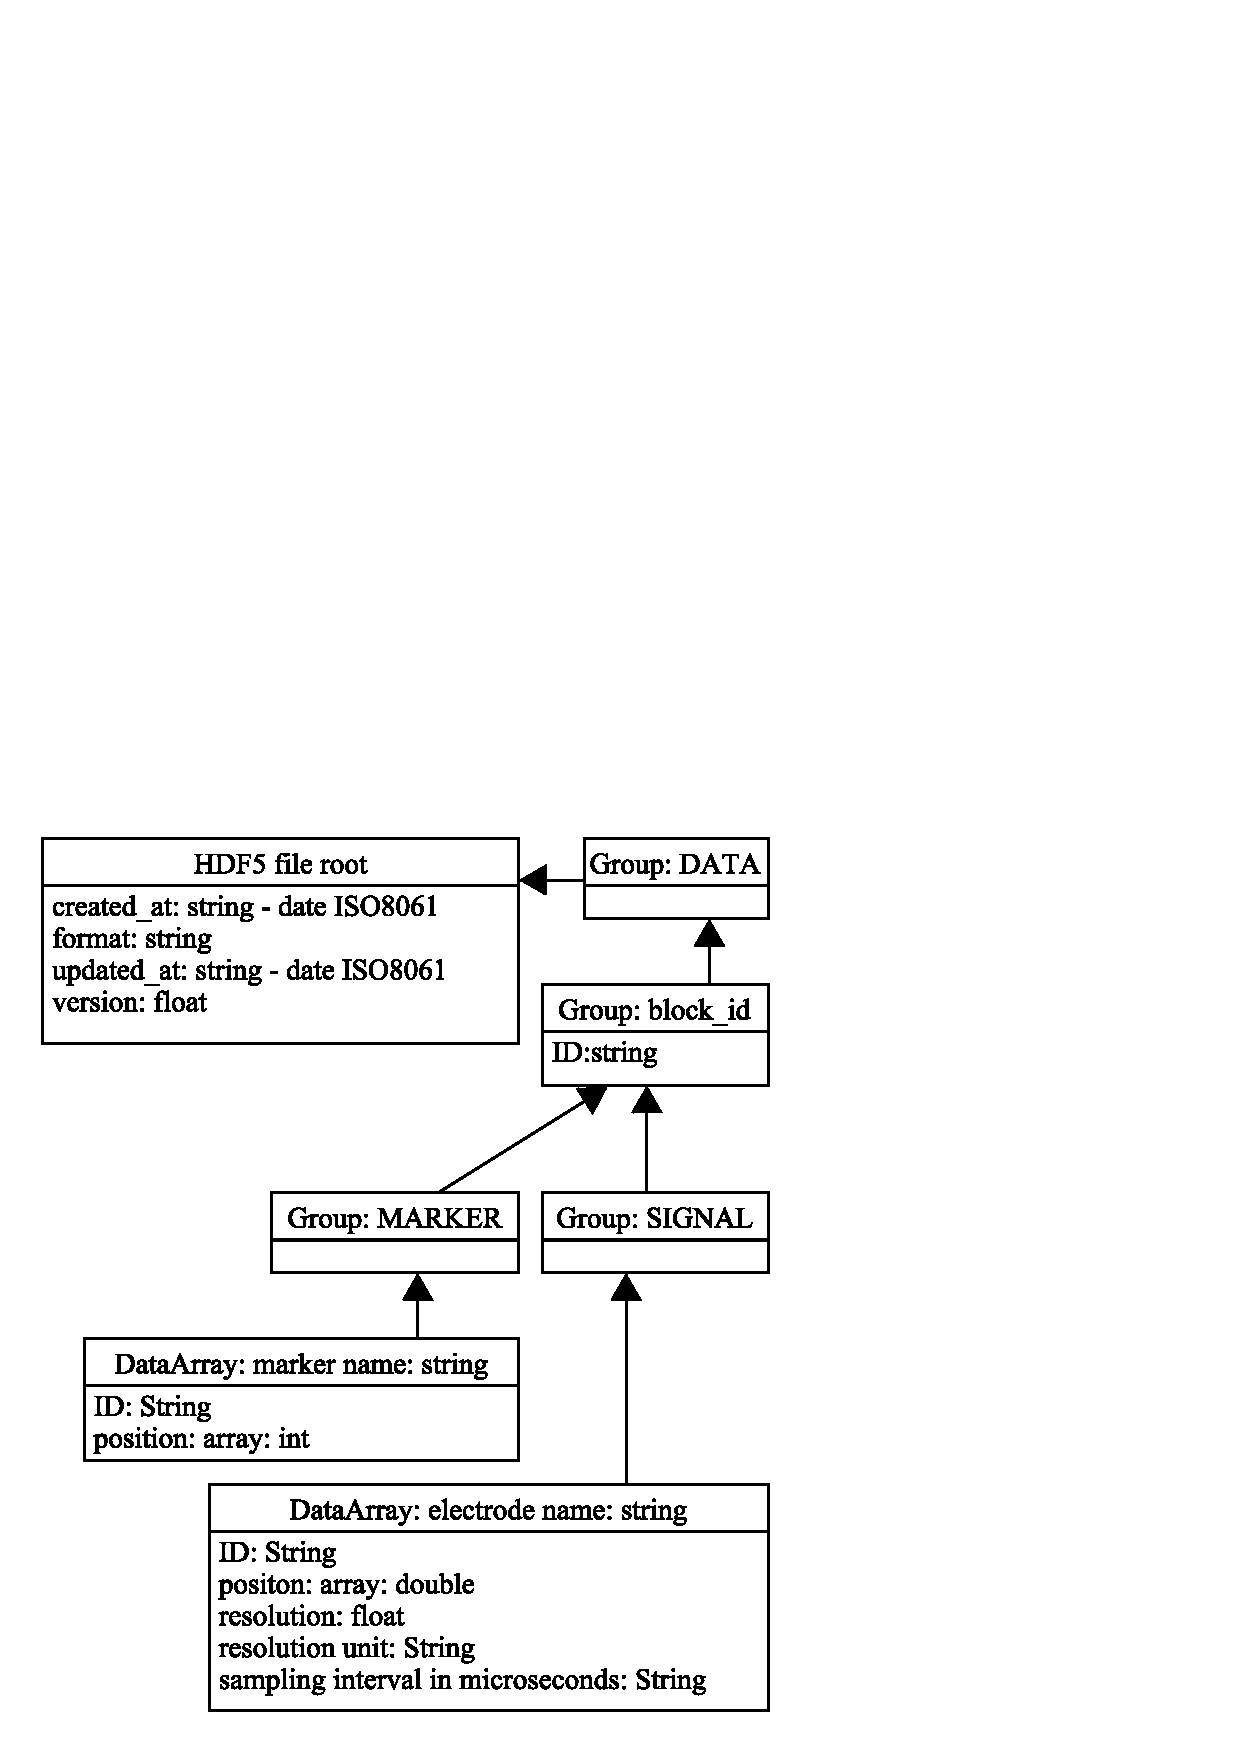
\includegraphics[scale=0.51]{obrazky/data.pdf}
		\caption{The final data model of proposed data format. The data are stored in tree structure with fixed terminology and structure. Each Group MARKER and SIGNAL could contain zero or more DataArrays with raw data.}
		\label{format_scheme}
	\end{center}
\end{figure}


\section{Model Ontology}
\subsection{Data Part}
Ontology and terminology of the data part is based on the NIX model that is described above in Section~\ref{section_data} - Data model and in Figure~\ref{format_scheme}.

\subsection{Metadata Part - odML}
\label{odml_section}
Metadata are organized according to \gls{odml} terminology. The \gls{gnode} \gls{odml} scheme and terminology was used for the metadata part of file, but there was some more information in the metadata scheme used at \gls{uwb}, which was difficult to save with existing \gls{odml} terminology. Therefore the \gls{odml} model and terminology were extended. The changes and adjustments are described in Section~\ref{meta_adjustments} - Metadata adjustments. We also decided that it would be useful to store some more data, which are more specific and could help to describe experiments better. The existing ontologies were also searched, for example Ontology for biomedical investigations \cite{oen} \cite{Brinkman2010}. However, I decided to use \gls{odml} because I was able to extend \gls{odml} to perfectly fit our needs and it is already used by the NIX model.


\subsection{UWB Metadata Model}
\label{meta_part}
This section shows all collected metadata, which are saved with experiments at \gls{uwb} and stored in the EEGBase portal \cite{eegportal}. The summary and comparison between the EEGBase portal information and original \gls{odml} (without our changes) model is in Table~\ref{comparsion}.

\newpage
\begin{longtable}{|l|l||l|l|}
	
\caption{The comparison between the EEGBase portal metadata model and terminology used by the odML model (without my adjustments).} \label{comparsion}\\
	\hline
	\multicolumn{2}{|c||}{\textbf{EEGBase}}& \multicolumn{2}{|c|}{\textbf{odML}} \\
	\hline 
	 \hline 
	\endfirsthead
	\multicolumn{4}{c}
	{\tablename\ \thetable\ -- \textit{Continued from previous page}} \\
	\hline	 
	\multicolumn{2}{|c||}{\textbf{EEGBase}}& \multicolumn{2}{|c|}{\textbf{odML}} \\
	\hline
	\hline  
	\endhead
	\hline \multicolumn{4}{c}{\textit{Continued on next page}} \\
	\endfoot
	\hline
	\endlastfoot
	 \hline Digitization & Gain & HW/Amplifier & Gain \\ 
	 \hline  Digitization & Filter & HW/Filter &  \\ 
 \hline 	 Digitization & Sampling\_rate & HW/DataAcq & SampleRate \\ 
 \hline 	 Pharmaceutical\footnote{Specification of pharmaceutics used by subject.} & Title & - &  \\ 
 \hline 	 Pharmaceutical & Description & - &  \\ 
 \hline 	 Artifact & Compensation & - &  \\ 
 \hline 	 Artifact & Reject\_condition	 & - &  \\ 
 \hline 	 Disease & Title & - &  \\ 
 \hline 	  Disease & Description & Subject & HealthStatus \\ 
 \hline 	 Weather & Description & - &  \\ 
 \hline 	 Weather & Title & - &  \\ 
 \hline 	 Artifact\_rem\_meth\footnote{Name of the used artifact remove method.} & Title & - &  \\ 
 \hline 	 Artifact\_rem\_meth\footnote{Description of the used artifact remove method.} & Description & - &  \\ 
 \hline 	 Software & Title & - &  \\ 
 \hline 	 Software & Description  & - &  \\ 
 \hline 	 Hardware & Title & HW/\textit{type}  & Model \\ 
 \hline 	 Hardware & Description &- &  \\ 
 \hline 	 Hardware & Type & - &  \\ 
 \hline 	 Project\_type & Title & Experiment & Type \\ 
 \hline 	 Project\_type & Description & - &  \\ 
 \hline 	 Subject\_group & Title &-  &  \\ 
 \hline 	 Subject\_group & Description & - &  \\ 
 \hline 	 Exper\_opt\_par\footnote{Name of optional experiment parameter.} & Param\_name & - &  \\ 
 \hline 	 Exper\_opt\_par\footnote{Data type of optional experiment parameter.} & Param\_type & - &  \\ 
 \hline 	 Exper\_opt\_par\_val\footnote{Value of optional experiment parameter.} & Param\_value & - &  \\ 
 \hline 	 Electrode\_conf & Impedance & Electrode & Impedance \\ 
 \hline 	 Electrode\_conf & Desc\_img\_ID & - &  \\ 
 \hline 	 Electrode\_system & Title & - &  \\ 
 \hline 	 Electrode\_system & Description & Electrode & ElectrodeCount \\ 
 \hline 	 Electrode\_location & Title & - &  \\ 
 \hline 	 Electrode\_location & Shortcut & - &  \\ 
 \hline 	 Electrode\_location & Description & - &  \\ 
 \hline 	 Electrode\_fix & Title & Electrode &  \\ 
 \hline 	 Electrode\_fix & Description & Electrode &  \\ 
 \hline 	 Electrode\_type & Title & Electrode & Type \\ 
 \hline 	 Electrode\_type & Description & Electrode &  \\ 
 \hline 	Scenario  & Title & - &  \\ 
 \hline 	Scenario  & Scenario\_Length & - &  \\ 
 \hline 	Scenario  & Description  & experiment/\textit{type} & Protocol \\ 
 \hline Scenario  & Scenario\_name & - &  \\ 
\hline Scenario  & Mimetype& - &  \\ 
\hline Stimulus & Description & Stimulus  & Desc/Start/End \\ 
	\hline Stimulus\_type & Description & - &  \\ 
	\hline Person & Givenname & Person & FirstName \\ 
	\hline Person & Surname & Person &LastName  \\ 
	\hline Person & Date\_of\_birth & Person & Birthday \\ 
	\hline Person & Gender & Person & Gender \\ 
	\hline Person & Email & Subject & ContactInfo \\ 
	\hline Person & Phone\_number & Subject & ContactInfo \\ 
	\hline Person & Note & Subject & Comment \\ 
	\hline Person & Laterality & - &  \\ 
	\hline Education\_level\footnote{Highest ducation level of person.} &Title  & - &  \\ 
	\hline Experiment & Start\_time & Recording & Start \\ 
	\hline Experiment &End\_time  & Recording & End \\ 
	\hline  Experiment& Temperature & - &  \\ 
	\hline  Experiment& Env\_note & - &  \\ 
	\hline  Experiment& Res\_group\_id & Recording & ExperimenterID \\ 
	\hline 
\end{longtable} 


\subsection{NIX Metadata Model}

The metadata model of NIX is using \gls{odml}. \gls{odml} is described in section \ref{odml_section}. The whole \gls{odml} terminology is too general and too extensive to list it here. So I chose the basic and most used sections which are related to our model and \gls{eeg} measurements and added it in Appendix~\ref{appendix1} in Figures~\ref{meta_scheme1}~\ref{meta_scheme2}~\ref{meta_scheme3}~\ref{meta_scheme4}. The EEGBase model contains modifications which are described below. 


\subsection{Metadata Terminology Extensions}
\label{meta_adjustments}
In order to save all our metadata into the \gls{hdf5} container I extended the \gls{odml} model for our metadata. These modifications were committed to \gls{gnode} respective \gls{incf} GitHub repository \cite{odmlgithub}. New sections \textbf{Environment}, \textbf{Protocol} and \textbf{Software} and several attributes to the existing sections \textbf{Person} and \textbf{Electrode} were added. All suggested changes were included into \gls{odml}. All modification are listed in Table \ref{modification}. Several attributes do not have descriptions, because their names are self-describing.
	\begin{longtable}{ | l | l | l | p{5cm} |}	
	\caption{Modifications of the \gls{odml} model.} 
	\label{modification}\\
\hline
\textbf{Name}& \textbf{Property} & \textbf{Value} & \textbf{Definition} \\
\hline 
\hline 
\endfirsthead
\multicolumn{4}{c}
{\tablename\ \thetable\ -- \textit{Continued from previous page}} \\
\hline	 
\textbf{Name}& \textbf{Property} & \textbf{Value} & \textbf{Definition} \\
\hline
\hline  
\endhead
\hline \multicolumn{4}{c}{\textit{Continued on next page}} \\
\endfoot
\hline

\endlastfoot
		Electrode & Usage & Ground & Usage of electrode. \footnote{Added terminology that describes usage of electrode.}\\
		\hline
		Electrode & Usage & Reference&Usage of electrode.\footnotemark[\value{footnote}] \\ 
		\hline
		Electrode & Usage & Channel& Usage of electrode.\footnotemark[\value{footnote}]\\ 
		\hline
		Electrode & Description & String& \\ 
		\hline		
		Environment & Weather & String & \\ 
		\hline	 
		Environment & RoomTemperature & String & \\ 
		\hline
		Environment & AirHumidity & float & The air humidity in \%.\\ 
		\hline
		Environment & Description & String &  \\ 
		\hline
		Protocol & Description & String & Description of the experiment\\ 
		\hline
		Protocol & Author & person & The persons who create this protocol.\\ 
		\hline
		Protocol & ProtocolFile & binary & Protocol File.\\ 
		\hline
		Protocol & ProtocolFileURL & URL & URL of protocol file.\\ 
		\hline
		Protocol & Version & String & Version of the protocol.\\ 
		\hline
		Person & Education level & String & Highest archived education level of the person.\\ 
		\hline
		Person & Role & Subject & The role of this person.\\ 
		\hline
		Person & Email & String & Person's e-mail.\\ 
		\hline
		Person & PhoneNumber & String & Person's phone number.\\ 
		\hline
		Person & Laterality & String & Handedness - The dominant hand of the subject.\\ 
		\hline
		Software & Name & String & The software name.\\ 
		\hline
		Software & Owner & String & The owner of software.\\ 
		\hline
		Software & Developer & String & Developer or developers firm of the software.\\ 
		\hline
		Software & Version & String & Version of the software.\\ 
		\hline
		Software & License & String & License type.\\ 
		\hline
		Software & LicenceStart & date & The start date of time limited license.\\ 		\hline
		Software & LicenceExpiration & date & The end date of time limited license.\\ 		\hline
		Software & LicenceDuration & String & Duration of the license for the software.\\ 		\hline
		Software & LicenceCount & int & Number of the software license.\footnote{For floating licenses}\\ 		\hline
		Software & Distribution & String & Distribution type.\\ 		\hline
		Software & Description & String & \\ 		\hline
		Software & LicenceDuration & String & Duration of the license for the software.\\ 		\hline
	\end{longtable} 

I also made some recommendations, which data would be useful to store a time zone, detail information about hardware and software and details about the project and experiments. The distribution of experiments by type in \gls{odml} is very useful and could be used in the EEGBase portal. The information about the project could be also helpful to identify a specific type of experiment. \gls{odml} is able to save most of these metadata and has a terminology for it so the EEGBase model is able to save them into the \gls{hdf5} container. When the current metadata model at University of West Bohemia will be extended it would not be problem to save it in EEGBase format. I suggested also that terminology of \gls{uwb} metadata model could use \gls{odml} terminology, because \gls{odml} have terminology for all currently saved information. 

\newpage
\subsection{EEGBase Metadata Model}
The model tree structure of EEGbase model metadata is in Appendix~\ref{appendix2}. Because \gls{odml} scheme is not mandatory but only recommended, it is possible to save, for example, experiments on mice which are also performed at \gls{uwb} in cooperation with The Faculty of Medicine - it is not necessary use both person and subject model, but it is possible to use only a subject's model. (Figure~\ref{person_vs_mouse}). The EEGBase model will store the tree structure of metadata into the EEGBase portal for easier, complete and adjustable metadata export.
\begin{figure}[h]
	\includegraphics[scale=0.6]{obrazky/person_vs_mouse.pdf}	
	\caption{The comparison of metadata sections for saving experiments with a person or a mouse.}
	\label{person_vs_mouse}
\end{figure}
\newpage
\section{HDFExport Program}
\subsection{Program Specification}
I chose the Java programing language because I was hoping to implement this program as a part of the EEGBase portal so it will be possible to export the data directly from the portal through an internet browser. This approach is similar to what Ovation uses (store information in database and allows export to \gls{hdf5}). The problems with \gls{hdf} libraries came up. Closer information about the EEGBase portal integration is in Section~\ref{integration}. The other option was to create a desktop application that uses \gls{soap} web services of EEGBase portal for loading data and metadata for export.

The program is designed for several use cases divided by data and metadata location (Figure~\ref{use_case1}):
\begin{itemize}
\item data and metadata export from locally stored Brain Vision files only
\item data and metadata export from locally stored Brain Vision files and metadata from EEGBase portal
\item data and basic metadata export from in EEGBase postal stored Brain Vision files without experiments metadata
\item data and metadata export from EEGBase portal and Brain Vision files stored in EEGBase portal
\end{itemize}

\begin{SCfigure}
	\includegraphics[scale=0.5]{obrazky/use_case_location.pdf}	
	\caption{Use cases of HDFExport Program.}
	\label{use_case1}
\end{SCfigure}
Other division is by type of exported data (Figure~\ref{use_case2}):
\begin{itemize}
	\item Only raw \gls{eeg} data and basic metadata are exported
	
	Only data and metadata from the Brain Vision files are exported. Stimuli are not exported (not all measurements uses stimuli).
	\item Raw \gls{eeg} data, basic metadata and stimuli are exported
	
	All data, metadata and stimuli from Brain Vision files are exported.
	\item Raw \gls{eeg} data, basic metadata, stimuli and experiments metadata are exported
	
	All data, metadata and stimuli from the Brain Vision files and experiments metadata from EEGBase portal are exported.
	\item Raw \gls{eeg} data, basic metadata and experiments information are exported
	
	All data, metadata and experiments information are exported.
\end{itemize}
\begin{SCfigure}
	\includegraphics[scale=0.5]{obrazky/use_case_data.pdf}	
	\caption{Use cases of HDFExport Program.}
	\label{use_case2}
\end{SCfigure}


\begin{figure}[h]
	\includegraphics[scale=0.73]{obrazky/ExportProgramDiagram.pdf}	
	\caption{The diagram of EEGBase HDF5 export program}
	\label{export-diagram}
\end{figure}

\subsection{Architecture}
The program for export is based on the three layer architecture. The Brain Vision files parser (EEGDataTransformer), web service client (EDEDClient), HDF5 writer (uses HDF Group libraries for work with \gls{hdf5} container) and \gls{gui} are the most important parts of the program. Some supportive classes were written (IDGenerator, IsoTime). These generate unique IDs and date in ISO format.



\chapter{Implementation}
This chapter describe the EEGBase format implementation and the EEGBase Export program implementation. 

\section{HDF Libraries}
\label{hdflib}
This section explains which libraries and \gls{hdf5} structures I used for \gls{hdf} file operation. 

The disadvantage is that the NIX project has no Java \gls{api} so it was necessary to use the \gls{hdf5} Java \gls{api} \cite{hdfjava}, but this \gls{api} is not native. The HDF Group creates several libraries for Java. The HDF-Java wrappers consist of the Java \gls{hdf} Object Package, related \gls{hdf4} and HDF5 Object Packages, and the native \gls{jhi} and \gls{jhi5}. The native interface includes the Java classes and C interface libraries.

The most intuitive way is using the HDF Object Package \cite{hdf_object}. But I wrote my application with \gls{jhi5} which is used by HDF Object Package, because it calls directly native C functions. Therefore the program should be more quick and also more examples are available (the Java functions are similar to C and Python functions). 

"The HDF Object Package does not provide a one-to-one mapping from Java methods to routines in the standard \gls{hdf4} and \gls{hdf5} libraries. The one-to-one mappings are provided via the HDF Java Native Interface products \gls{jhi} and \gls{jhi5}. The HDF Object Package wraps these direct mappings with a higher level object model." \cite{hdf_object} The diagram is in Figure~\ref{hdf-obj}.

\begin{SCfigure}
	\includegraphics[scale=0.49]{obrazky/hdf-obj.jpg}
	\caption{The HDF Object Package. \cite{hdf_object}}
	\label{hdf-obj}
\end{SCfigure}

The \gls{hdf} works with five basic types of objects:

\begin{itemize}
	\item \textbf{Group}
	
A group is used as a folder in the file system, it divides objects into the logical groups. The group can contain none or more objects and can be member of another group.
\newpage
	\item \textbf{Dataspace}
	
This is a required part of \gls{hdf5} Dataset or Attribute. The Dataspace contains raw data and defines size and shape of data (defines the number of dimensions and size of each element).
	\item \textbf{Dataset}
	
	The Dataset is an object that describes stored data. It could contain none or more attributes and it is composed from raw data, metadata, data layout or other information necessary to write, read or interpret the stored data. The application view of a dataset is in Figure~\ref{dataset_figure}.	
	\begin{figure}[h]
		\begin{center}
			\includegraphics[scale=0.6]{obrazky/dataset.jpg}
			\caption{Application view of a dataset. \cite{hdf}}
			\label{dataset}
		\end{center}
	\end{figure}
		\begin{figure}[h]
			\begin{center}
				\includegraphics[scale=0.7]{obrazky/dataset-with-att.PNG}
				\caption{Example of HDF5 file with EEGBase format in HDFView 2.11- the Dataset with name T6 (EEG channel) with Dataspace (array of 1414260 double numbers) and four attributes.}
				\label{dataset_figure}
			\end{center}
		\end{figure}
	\item \textbf{Datatype}
	
The \gls{hdf5} datatype defines the storage format for a single data element. The description is in Figure~\ref{datatype}. The datatype describes the storage layout of a single data element. All elements of the dataset must have the same type and the datatype of a dataset is immutable.
	\begin{figure}[h]
	\centering
		\includegraphics[scale=0.7]{obrazky/datatype.jpg}
		\caption{Datatypes, dataspaces, and datasets. \cite{hdf}}
		\label{datatype}	
\end{figure}

\newpage
	\item \textbf{Attribute}
	
	An \gls{hdf5} attribute is a small metadata object describing the nature and/or intended usage of a primary data object. A primary data object may be a dataset, group. Even though an attribute is not a standard \gls{hdf5} Dataset, it has several common properties: \cite{hdf}
	\begin{itemize}
\item An attribute has a user-defined dataspace and the included metadata has a user-assigned datatype
\item Metadata can be of any valid HDF5 datatype
\item Attributes are addressed by name
	\end{itemize} 
	Attributes are from Datasets different in:
		\begin{itemize}
			\item There is no provision for special storage such as compression or chunking
			\item There is no partial I/O or sub-setting capability for attribute data
			\item Attributes cannot be shared
			\item Attributes cannot have attributes
			\item Attributes are stored in the object header
		\end{itemize} 
\end{itemize}

Since all elements defined in \gls{hdf5} have names, they can be referenced by their path. \cite{pandora2}

\section{Used HDF5 Data Types}

The following data types were used in the \gls{hdf5} container:

\begin{itemize}
	\item \textbf{double} 
	
	The signal raw data are stored as the \gls{hdf5} type H5T\_IEEE\_F64LE.
	\item \textbf{float}
	
	Float numbers are saved as the \gls{hdf5} type H5T\_IEEE\_F32LE. The stimuli raw data are saved in this format.
	\item \textbf{string} 
	
	All strings are stored as type H5T\_C\_S1. Almost all attributes, dates and IDs are saved as strings.
	
\end{itemize}

\section{EEGBase File Structure}

The root of the file contains basic information about the file and the format. It also divides the file container into two groups Data and Metadata. (Table~\ref{file_root}). The \gls{iso} 8601 format was used for the date, because even though \gls{hdf5} has a data type for the date, it is not platform independent. The NIX model does not have the date format specified so I chose the norm of \gls{ecsn} \gls{iso} 8601 \cite{iso8601}, which is one of many possible formats and it is the Czech version of the international format \gls{iso} 8601:2004. This norm allows the user to save date and time at once and specify even the time zone. This could be important for the flawless representation of measured data. Then the final Date string is: Complete date plus hours, minutes, seconds and a decimal fraction of a second YYYY-MM-DDThh:mm:ss.sTZD (e.g. 1997-07-16T19:20:30.45+01:00) \cite{iso8601}. This date and time is saved as String so it is platform independent and thanks to the \gls{iso} norm is standardized.


Recordings are wrapped into the blocks (HDF groups). Each recorded channel with basic metadata is saved in a block. The recorded signal values (raw data) are stored in the Dataset with the name of the channel. Information from files eeg (Section~\ref{eeg}) (raw data) and vhdr (Section~\ref{vhdr}) (metadata) and generated IDs are stored in the DATA section.
Markers (stimuli and artifacts etc.) information are stored in a block in the section MARKERS and they are saved also in the Datasets with the name of the marker. (Figure~\ref{datasection_exp}).
\begin{table}
	\begin{tabular}{l l l}
		root &  & \\ 
		\hline attribute & format & string \\ 
		attribute & version & string \\ 
		attribute & created\_at & string - date ISO 8601 \\ 
		attribute & updated\_at & string - date ISO 8601\\ 
		\hline	 group &  DATA & \\ 
		group & METADATA & \\ 
		\hline	 
	\end{tabular} 
	\caption{The root of \gls{hdf5} file.} 
	\label{file_root}
\end{table}

\begin{SCfigure}[][h]
		\includegraphics[scale=0.8]{obrazky/data-section.png}
		\caption{Example of HDF5 file with EEGBase format in HDFView 2.11- the DATA section.}
		\label{datasection_exp}

\end{SCfigure}

The \gls{hdf5} container stores information about array dimensionality and a stored data type natively. (Figure~\ref{dataset_figure}).

\section{HDFExport Program Modules}

\subsection{Brain Vision Files Parser}
The EEGDataTransformer from Jan Štěbeták \cite{eegloader} was used as a parser for current eeg, vhdr and vrmk files.  Only minor changes of this program were made. I added the class AmplifierInfo and ImpedanceInfo and the methods NumberOfChannels, SamplingInterval, getAmplifier, getImpedanceInfo into DataTransformer interface. The method getUnits() of ChannelInfo class was edited, because the returned String was in wrong format. Figure~\ref{eegexport}.

\begin{figure}
	\includegraphics[scale=0.75]{obrazky/EEGExport.png}
	\caption{Class diagram of edited EEGDataTransformer program. New methods and classes are marked.}
	\label{eegexport}
	
\end{figure}

\subsection{Metadata Loader}
The metadata are loaded through web services, which were written by Jan Štěbeták \cite{webservice}, and from Brain Vision vhdr file.

The program uses the web service UserDataService and its methods for loading all experiments metadata.
The client was generated from \gls{WSDL} file \cite{wsdl}. EDEDCLient \cite{jerpa} written by Petr Miko was used as a client for web services.

\subsection{HDF5 Writer}
The writer consists of three classes:
\begin{itemize}
	\item HDF5file
	
	The the \gls{hdf5} file is created in this class and all necessary information about format (Version, Format name, Date) are written in the file. This class uses and calls methods from DataWriter and MetaDataWriter classes.
	
	\item DataWriter
	
	This class saves all binary data and markers to the \gls{hdf5} container. This class saves also essential metadata of raw data into attributes.
	
	\item MetaDataWriter
	
	This class stores all loaded metadata into METADATA part (Section~\ref{meta_part}).
	
\end{itemize}

\begin{figure}
	\begin{center}
		\includegraphics[scale=0.4]{obrazky/HDF5_file.jpg}
		\caption{HDF5 file with data with EEGBase format - in HDFView 2.11}
		\label{hdf5_file}
	\end{center}
\end{figure}

The programming was not simple, because the C methods stayed the same and the wrappers only allow to be called from Java Virtual Machine. The example of the Java code and calls of C functions are in Listing~\ref{java2}.
The methods for easier work with \gls{hdf5} libraries were written and the code for saving string into the \gls{hdf5} file is in Listing~\ref{stringsave} and for storing binary data into the datasets is in Listing~\ref{java3}.

\definecolor{dkgreen}{rgb}{0,0.6,0}
\definecolor{gray}{rgb}{0.5,0.5,0.5}
\definecolor{mauve}{rgb}{0.58,0,0.82}

\lstset{frame=tb,
	language=Java,
	aboveskip=3mm,
	belowskip=3mm,
	showstringspaces=false,
	columns=flexible,
	basicstyle={\small\ttfamily},
	numbers=none,
	numberstyle=\tiny\color{gray},
	keywordstyle=\color{blue},
	commentstyle=\color{dkgreen},
	stringstyle=\color{mauve},
	breaklines=true,
	breakatwhitespace=true,
	tabsize=3
}
\newpage
\begin{lstlisting}[language=C,frame=single,caption={Creating Group in HDF5 with Java wrappers. This code creates a new group with the name METADATA at the specified location block},label=java2]
//create Group
H5.H5Gcreate(this.block, "METADATA", HDF5Constants.H5P_DEFAULT, HDF5Constants.H5P_DEFAULT, HDF5Constants.H5P_DEFAULT);

\end{lstlisting}

\begin{lstlisting}[language=C,frame=single,caption={Saving binary data into the dataset. It saves H5T\_IEEE\_F64LE (double) in dset\_data if saving location dataset\_id exists},label=java3]
if (dataset_id >= 0) // location exists
H5.H5Dwrite(dataset_id, HDF5Constants.H5T_IEEE_F64LE, HDF5Constants.H5S_ALL, HDF5Constants.H5S_ALL, HDF5Constants.H5P_DEFAULT, dset_data);
\end{lstlisting}

\begin{lstlisting}[language=C,frame=single,caption={Saving string as attribute in HDF5.},label=stringsave]
//SaveString method
int attribute_space,attribute_id=-1;
int stype =-1;
//create space for one char
attribute_space = H5.H5Screate(HDF5Constants.H5S_SCALAR);
//copy size of char
stype = H5.H5Tcopy(HDF5Constants.H5T_C_S1);	
//sets size of string lenght*size of char
H5.H5Tset_size(stype, savedString.length());
//create attribute in location dataset_id, with name HdfName, size stype
attribute_id = H5.H5Acreate(dataset_id, HdfName, stype, attribute_space, HDF5Constants.H5P_DEFAULT, HDF5Constants.H5P_DEFAULT);
//writes string into prepared attribute_id, with size of stype
H5.H5Awrite(attribute_id, stype, savedString.getBytes());	
//if all was correct close space	
if(attribute_space>-1){
  H5.H5Sclose(attribute_space);
}
//if all was correct close attribute	
if(attribute_id>-1){
  H5.H5Aclose(attribute_id);
}

\end{lstlisting}




\subsection{Graphical User Interface}
The program has only a basic \gls{gui}, because the main purpose is to provide methods for saving all current data and metadata to the \gls{hdf5} container. The methods which are working with \gls{hdf5} container are general and it is possible to use them in any other program. All methods are in separate classes in a special package hdf5. \gls{gui} for locally stored data use case is presented in Figure~\ref{program-gui}.

\begin{figure}[h]
	\begin{center}
		\includegraphics[scale=0.7]{obrazky/program_gui2.PNG}
		\caption{EEGBase HDF5 export program. Metadata are loaded trough web services.}
		\label{program-gui}
	\end{center}
\end{figure}

\section{EEGBase Portal Integration}
\label{integration}
Although my first effort was to import my program into the EEGBase portal, I was unable to do so. I tried to create a prototype which would save stored data into the \gls{hdf5} file in a web container. However I could not make Java wrappers work in the web container. I contacted \gls{hdf} Group support for advice, however, the support and developers did not know how to develop such a program. I did some research and I tried to make the program work on the Tomcat server and Glassfish server but with no success. For those reasons I chose to use the EEGBase portal \gls{soap} web services to load data for export to the \gls{hdf5} container.

It was necessary to create a new web service, which will export all metadata of the experiment. The web service \textit{getExperimentsMetadata} was created for that reason and it is used by my program.


\chapter{Tests}

The program was manually tested for several use cases and all created \gls{hdf5} files were verified manually (opened and the contents was checked) by official program of HDF Group HDFView \cite{hdfjava} in version 2.11 - Figure~\ref{hdf5_file}. The following test describing writing speed into \gls{hdf5} container were conducted. (Table~\ref{speed_test}). The file size of created files were also tested. (Table~\ref{file_size}).



\section{Performance Tests}

The write performance tests were conducted to determine time consumption of export. The tests were conducted on a standard desktop computer (processor Intel Core i7 at 3,4 GHz, 8 GB of DDR3 RAM, standard HDD with 7200 rpm). An unusually high memory consumption was detected during the test. The amount of occupied memory by the EEGExport program for big (220 MB) measurements reached up to 4 GB of memory. Further testing showed that Java Virtual Machine, in attempt to speed up export, does not free allocated memory. However, if the program was paused the amount of allocated memory was lower; the program could run with less memory. In the end the disk writing speed was a limited factor. The conversion times with GZip compression are shown in Table~\ref{speed_test}.

\begin{table}
	 \catcode`\-=12
	\centering
	\caption{Performance tests with GZip compression. Each file was saved seven times.}
	\label{speed_test}
	\begin{tabular}{|c|c|c|c|c|}
		\hline
\textbf{File size} & \multicolumn{4}{c|}{\textbf{Time needed for conversion in ms}}\\ 
	\cline{2-5}		
	\textbf{ of Brain Vision files}	&\textbf{Best} & \textbf{Worst} & \textbf{Average} & \textbf{With compression\footnote{Average time from four savings.}}\\ 
	\hline
				\hline 21,3 MB & 3010 & 3501  & 3132& 7529 \\ 	
			\hline 51,2 MB & 6160  & 7906 & 6700 & 26051\\ 
				\hline 58 MB & 7668 &  8262 &  7947& 29032\\ 
			\hline 87,2 MB & 31364 & 35957 & 32820& 44877\\ 
			\hline 197,8 MB & 13060  & 14625 &  13502& 40168\\ 		
			\hline 221,3 MB & 14589 & 16321 & 15197& 42679 \\ 
			\hline 221,6 MB & 14347  & 16108 & 14871& 43586\\ 
		\hline 
	\end{tabular} 
\end{table}
	\footnotetext{Average time from four savings.}

\section{File Size Test}
Several test were conducted to determine the resulting file size of the \gls{hdf5} container containing all data. Data from real experiments were used for the tests. The test shows that size of the \gls{hdf5} container is influenced by exported data and the original file size is not the only decisive factor. The size of the \gls{hdf5} container is always bigger then Brain Vision files, at worst case even four times bigger in the best scenario about two times bigger. The results are shown in Table~\ref{file_size}. The ratio is better for longer and bigger measurements. The GZip compression was used to reduce file size. The GZip compression is integrated in \gls{hdf} libraries and it is supported natively (reading of the data does not require any special actions). The size of compression chunk was set to 256 after several tests. The file size was decreasing with bigger chunk size, but the performance was decreasing. This settings had the best results in file size compared to the impact on performance. With the GZip compression the file size ratio decreased to 1,62 in average. The influence of chunk size on file size is in Table~\ref{chunk_size}. The comparison between GZip and SZip compression is in Table~\ref{compression}. The GZip compression is better for smaller experiments. With bigger data the SZip compression gets a smaller final file. However, most of experiments have smaller size (smaller than 100 MB) I chose the GZip compression as default compression algorithm.

\begin{table}[h]
\caption{File size tests.}
\label{file_size}
\centering
\begin{tabular}{|c|c|c|c|}
	\hline \textbf{File size}  & \multirow{2}{*}{\textbf{HDF5 file size}}& \multirow{2}{*}{\textbf{HDF5 file size}}  & \textbf{Ratio} \footnote{(HDF5 is x times bigger)}	\\
		\textbf{of Brain Vision files} & &  with compression &	\\ 
			\hline 21,3 MB & 80,9 MB & 26,92 MB& 1,26x\\ 
	\hline 51,2 MB & 194,2 MB & 112,98 MB & 2,21x\\
		\hline 58 MB & 221,1 MB & 102,79 MB & 1,77x\\  
	\hline 87,2 MB & 329,7 MB & 124,51 MB & 1,43x\\ 
	\hline 197,8 MB & 370,9 MB & 305,19 MB& 1,54x\\ 


	\hline 221,3 MB & 414,9 MB & 355,58 MB & 1,61x\\ 
		\hline 221,6 MB & 415,5 MB & 334,46 MB & 1,51x\\ 
	
	\hline 
\end{tabular} 
\end{table}
\footnotetext{HDF5 is x times bigger than original file size.}
\begin{table}
	\caption{File size dependency on compression chunk size.}
	\label{chunk_size}
	\centering
	\begin{tabular}{|c|c|c|c|c|}
		\hline \multirow{2}{*}{\textbf{Original file size}}  & \multicolumn{4}{ c| }{\textbf{HDF5 file size in MB}}\\
		 & chunk 64 & chunk 256 & chunk 512 &  chunk 1024	\\ 
		 	\hline 21,3 MB &  39,76  & 26,92 & 23,30 & 20,46\\ 	
		\hline 51,2 MB & 155,47 & 112,98  & 99,31 & 87,85 \\ 
		\hline 58 MB    & 151,31 & 102,79 & 88,60 & 77,96 \\ 
		\hline 87,2 MB & 176,53  & 124,51 &  112,43& 104,15\\ 
		\hline 197,8 MB & 365,63 & 305,19 & 292,59 & 285,48\\ 		
		\hline 221,3 MB & 422,83  & 355,58& 341,72 & 333,83\\ 
		 \hline 221,6 MB & 402,81 & 334,46 & 320,22 & 312,10 \\ 
		\hline 
	\end{tabular} 
\end{table}

\begin{table}
	\caption{File size dependency on compression method. The chunk size is 256.}
	\label{compression}
	\centering
	\begin{tabular}{|c|c|c|}
		\hline \textbf{Original file size}  & \textbf{File size with SZip} & \textbf{File size with GZip}\\
		\hline 21,3 MB &  33,51 MB & 26,92 MB\\ 
		\hline 51,2 MB & 138,01 MB& 112,98 MB \\ 
		\hline 58 MB    & 148,88 MB& 102,79 MB \\ 
		\hline 87,2 MB & 145,53 MB & 124,51 MB \\ 
		\hline 197,8 MB & 280,92 MB& 305,19 MB \\ 
		\hline 221,3 MB & 331,01 MB & 355,58 MB\\ 
		\hline 221,6 MB & 306,03 MB& 334,46 MB  \\	
		\hline 
	\end{tabular} 
\end{table}